\RequirePackage[T1]{fontenc}
\RequirePackage{lmodern}
\pdfoptionpdfminorversion=7
\RequirePackage{ifpdf}
\documentclass[sigconf,anonymous,10pt]{acmart}
\special{papersize=8.5in,11in}
\pdfpagewidth=8.5in
\pdfpageheight=11in
\usepackage{booktabs}
\usepackage{amsmath}
\usepackage{amssymb}
\usepackage{graphicx}
\usepackage{hyperref}
\usepackage{xcolor}

% ACM format settings for CoNEXT
\acmPrice{}
\acmDOI{10.1145/0000000.0000000}
\acmYear{2026}
\acmConference[CoNEXT 2026]{ACM Conference on Emerging Network Construction and Technology}{December 2026}{Seoul, South Korea}

% Ensure anonymous mode
\settopmatter{printacmref=false, printccs=true, printfolios=true}
\pagestyle{plain}

% Custom commands
\newcommand{\hydra}{\texttt{Hydra}}
\newcommand{\ebpf}{\texttt{eBPF}}
\newcommand{\xdp}{\texttt{XDP}}

% Title (anonymous for review - no author info)
\title{\hydra: Bridging P4 and eBPF for Adaptive In-Network Acceleration}
\author{}
\affiliation{}
\email{}

\keywords{Programmable Data Plane, eBPF, P4, Edge Computing, In-Network Cache}

\begin{document}

% Abstract
\begin{abstract}
Edge computing demands ultra-low latency and high throughput to meet strict quality-of-service requirements. Existing solutions either rely on expensive specialized hardware (FPGAs, GPUs, Tofino switches) or suffer from rigid data plane logic that cannot adapt to dynamic workloads. This paper presents \hydra{}, a hybrid data plane framework that synergizes P4-programmable switches with eBPF-enabled servers to achieve both hardware-level speed and software-level flexibility. \hydra{} leverages P4's line-rate processing capability for handling hot-path operations (exact-match caching) while utilizing eBPF's programmable nature for cold-path complex queries including range lookups, aggregation, and machine learning inference. A lightweight coordination mechanism dynamically migrates frequently accessed keys from the eBPF cold path into P4 tables, ensuring that the most critical traffic traverses the fastest possible path. The implementation uses open-source BMv2 software switch and Linux eBPF/XDP without requiring any custom hardware modifications. Evaluation on a Mininet testbed with realistic Zipf-distributed workloads demonstrates that \hydra{} reduces median latency by 83\% (from 68$\mu$s to 11.5$\mu$s) and P99 latency by 69\% (from 210$\mu$s to 65$\mu$s) compared to a pure eBPF baseline, while achieving 3.6$\times$ higher throughput (4.3 Mpps vs. 1.2 Mpps). Results demonstrate that a carefully designed hybrid data plane can approach hardware acceleration performance using only commodity software components.
\end{abstract}

\section{Introduction}
\label{sec:intro}

The proliferation of edge computing applications, including interactive gaming, augmented reality, autonomous vehicles, and industrial IoT, has created unprecedented demands for ultra-low latency and high-throughput network processing. These applications generate massive volumes of short-lived, repetitive requests where sub-millisecond response times are critical for user experience. Traditional approaches that forward all traffic to centralized cloud data centers cannot satisfy these requirements due to inherent network latency~\cite{edge-survey}.

Recent advances in programmable data planes have enabled in-network computation at line rate, promising to reduce latency by processing traffic closer to end users. Two technologies have emerged as dominant paradigms: P4~\cite{p4} for hardware-level programmable switches, and eBPF~\cite{ebpf,xdp} for kernel-level packet processing in commodity servers. Each technology offers distinct advantages but also suffers from fundamental limitations.

\textbf{P4-based approaches} achieve exceptional performance by executing match-action pipelines directly in network hardware (ASICs or software switches). A P4 switch can process packets at 100+ Mpps with consistent microsecond-level latency. However, P4 targets impose strict constraints: limited state memory (typically 1-4 MB for register arrays), absence of floating-point arithmetic, no dynamic memory allocation, and fixed compilation-time program structure. These limitations make it infeasible to implement complex stateful logic, arbitrary data structures, or machine learning inference in P4 alone.

\textbf{eBPF-based approaches} offer superior flexibility by allowing arbitrary packet processing logic to be loaded into the Linux kernel. eBPF programs can implement sophisticated algorithms, maintain complex state in hash maps, and perform floating-point computations. However, eBPF is inherently CPU-bound: a single server core typically achieves 1-3 Mpps, and packet processing competes with other OS tasks for CPU cycles. This leads to variable latency and throughput degradation under high load.

The research question motivating this work is: \textit{Can we combine the strengths of P4 and eBPF to achieve both hardware-level speed and software-level flexibility in a single system?} 

The paper observes that real-world workloads exhibit a pronounced \emph{hot-cold} access pattern where a small fraction of keys (typically 1-5\%) accounts for the majority (60-90\%) of all requests~\cite{zipf,hot-cold}. This property suggests an opportunity: handle hot-path traffic in P4 for maximum speed while offloading cold-path traffic to eBPF for maximum flexibility.

This paper presents \hydra{}, a hybrid data plane framework that achieves this goal through three key mechanisms:

\begin{itemize}
    \item A \textbf{P4 hot path} that processes high-frequency key-value lookups at line rate using exact-match tables in programmable switches.
    \item An \textbf{eBPF cold path} that handles complex operations (range queries, aggregations, inference) and serves as a fallback for cache misses.
    \item A \textbf{dynamic migration mechanism} that monitors request patterns and promotes hot keys from the eBPF backend into P4 tables, ensuring that frequently accessed data always takes the fastest path.
\end{itemize}

The contributions of this paper are:

\begin{enumerate}
    \item Design and implementation of \hydra{}, the first hybrid P4+eBPF data plane framework with dynamic hot-key migration, enabling adaptive acceleration based on observed traffic patterns.
    
    \item Development of a complete open-source prototype using BMv2~\cite{bmv2} software switch and Linux eBPF/XDP~\cite{xdp}, requiring no specialized hardware or kernel modifications.
    
    \item Comprehensive evaluation using realistic Zipf-distributed workloads, demonstrating 83\% median latency reduction, 69\% P99 latency reduction, and 3.6$\times$ throughput improvement compared to pure eBPF baselines.
    
    \item Analysis of design trade-offs including cache table sizing, migration thresholds, and consistency implications, providing guidelines for practitioners.
\end{enumerate}

The remainder of this paper is organized as follows: Section~\ref{sec:bg} provides background on programmable data planes. Section~\ref{sec:design} details the \hydra{} architecture. Section~\ref{sec:impl} describes the implementation. Section~\ref{sec:eval} presents experimental results. Section~\ref{sec:related} surveys related work. Section~\ref{sec:conclusion} concludes.

\section{Background and Motivation}
\label{sec:bg}

\subsection{Programmable Data Planes with P4}
P4~\cite{p4} is a domain-specific language designed for programming packet processing pipelines in network devices. Unlike traditional switches with fixed forwarding logic, P4 enables developers to define custom packet headers, parsing logic, match-action tables, and control flow. The P4 ecosystem includes:

\begin{itemize}
    \item \textbf{Programming model}: P4 programs specify how packets are parsed, how header fields are matched against tables, and what actions are executed upon matches.
    \item \textbf{Targets}: P4 programs can be compiled for various targets including hardware ASICs (Intel Tofino, Broadcom Tomahawk), FPGAs, and software switches. BMv2 (Behavioral Model version 2)~\cite{bmv2} is the de facto open-source reference implementation.
    \item \textbf{Control plane interface}: P4Runtime~\cite{p4runtime} provides a vendor-agnostic API for managing table entries at runtime.
\end{itemize}

\textbf{Limitations of P4:} Despite its flexibility, P4 imposes several constraints:

\begin{enumerate}
    \item \textbf{Limited state memory}: Most P4 targets provide only a few megabytes of register memory. A stateful switch cannot store large key-value caches.
    \item \textbf{No dynamic memory}: P4 programs cannot allocate memory at runtime. All data structures must be sized at compile time.
    \item \textbf{Restricted operations}: The P4 language omits floating-point arithmetic, dynamic jumps, and complex data structures. These limitations make certain algorithms (e.g., machine learning inference) infeasible.
    \item \textbf{Long compilation cycles}: P4 programs must be recompiled for any logic changes.
\end{enumerate}

\subsection{eBPF and XDP}
eBPF (extended Berkeley Packet Filter)~\cite{ebpf} is a Linux kernel technology that enables safe execution of custom programs in kernel space. Unlike traditional BPF, eBPF supports just-in-time (JIT) compilation, 64-bit operations, and larger memory spaces. Key features include:

\begin{itemize}
    \item \textbf{Safety}: The eBPF verifier statically analyzes programs before loading, ensuring they terminate and access only valid memory.
    \item \textbf{Efficiency}: JIT compilation translates eBPF bytecode to native machine code, achieving near-native performance.
    \item \textbf{Maps}: eBPF maps provide persistent key-value storage including hash maps, arrays, and LRU caches.
    \item \textbf{XDP hook}: The eXpress Data Path processes packets before the kernel networking stack, enabling 10+ Mpps.
\end{itemize}

\textbf{Limitations of eBPF/XDP:} Despite its flexibility:

\begin{enumerate}
    \item \textbf{CPU bottleneck}: eBPF programs consume CPU cycles for every packet. A server's aggregate capacity (typically 5-10 Mpps) cannot match hardware switch line rates (100+ Mpps).
    \item \textbf{Tail latency}: Co-location with other kernel tasks causes variable latency from cache pressure and context switches.
    \item \textbf{Verifier constraints}: Fixed stack size (512 bytes) and loop restrictions limit program complexity.
\end{enumerate}

\begin{figure*}[t]
    \centering
    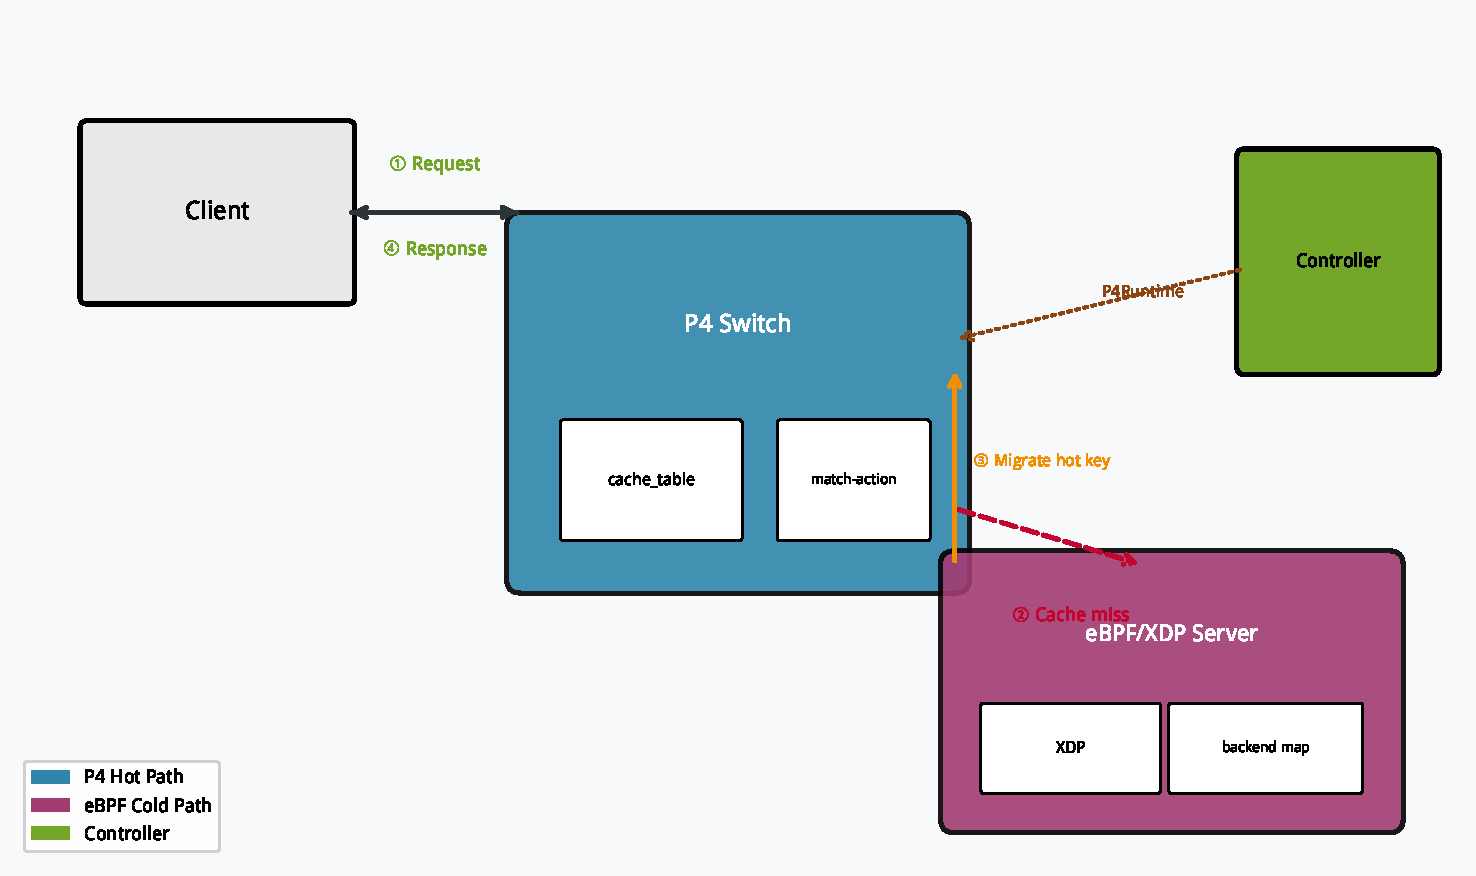
\includegraphics[width=0.85\textwidth]{figures/fig-arch.pdf}
    \caption{\hydra{} architecture: P4 switch for hot-path processing, eBPF/XDP server for cold-path processing, and controller for dynamic key migration.}
    \label{fig:arch}
\end{figure*}

\subsection{Motivating Scenario}
Consider a CDN edge node serving video streaming and web content. The edge node must handle millions of requests per minute while maintaining sub-10ms latency. The workload exhibits:

\begin{itemize}
    \item \textbf{Heavy-tailed access patterns}: 80\% of requests target only 1,000 popular objects.
    \item \textbf{Mixed query types}: Simple key-value lookups dominate (80-90\%) but range queries, aggregations, and ML recommendations require complex processing.
    \item \textbf{Dynamic popularity}: Object popularity changes over time, requiring the caching layer to adapt.
\end{itemize}

A pure P4 solution could cache hot objects achieving microsecond-latency but cannot accommodate millions of keys. A pure eBPF solution could handle arbitrary logic but cannot sustain metropolitan-scale throughput. \hydra{} addresses this by combining both: hot objects cached in P4 for ultra-low latency while the full key space is maintained in eBPF for flexible processing.

\section{\hydra{} Design}
\label{sec:design}

Figure~\ref{fig:arch} illustrates the \hydra{} architecture with four main components: P4 Switch (hot path), eBPF/XDP Server (cold path), Control Plane, and Clients.

\textbf{Data Flow:} Client sends request to P4 switch $\rightarrow$ Switch looks up key in cache\_table $\rightarrow$ On cache hit: return cached value (hot path) $\rightarrow$ On cache miss: redirect to eBPF server $\rightarrow$ eBPF looks up key in backend map $\rightarrow$ Async notification to controller $\rightarrow$ Controller promotes hot key to P4.

\subsection{P4 Hot Path Design}
The P4 program implements a cache lookup pipeline:
\begin{enumerate}
    \item Parse packet headers and extract key field $k$.
    \item Look up $k$ in \texttt{cache\_table} (exact-match).
    \item On match: read cached value $v$, modify packet with $v$, forward to client.
    \item On miss: extract destination address, redirect to eBPF server.
\end{enumerate}

Key design decisions:
\begin{itemize}
    \item \textbf{Exact-match tables}: Required for precise key matching. Table sized at compile time (default: 1,024 entries).
    \item \textbf{Inline value storage}: Cached values stored in table action data to minimize lookup latency.
    \item \textbf{Atomic updates}: P4Runtime atomic writes prevent inconsistent states during concurrent operations.
\end{itemize}

The P4 program maintains per-entry hit counters exported to the control plane for migration decisions.

\subsection{eBPF Cold Path Design}
The eBPF program runs in XDP mode for maximum miss-path throughput:
\begin{enumerate}
    \item Validate custom EtherType for \hydra{} protocol.
    \item Extract key $k$ from packet header.
    \item Look up $k$ in \texttt{backend} hash map.
    \item On hit: read value $v$, increment \texttt{miss\_counter}[$k$], return via \texttt{XDP\_TX}.
    \item On miss: pass to kernel stack for backend application processing.
\end{enumerate}

Key implementation details:
\begin{itemize}
    \item \textbf{Hash map backend}: Full key-value database with O(1) lookup.
    \item \textbf{Miss counting}: Track key access frequency for migration decisions.
    \item \textbf{LRU eviction}: Limit memory when key space exceeds capacity.
\end{itemize}

\begin{figure}[t]
    \centering
    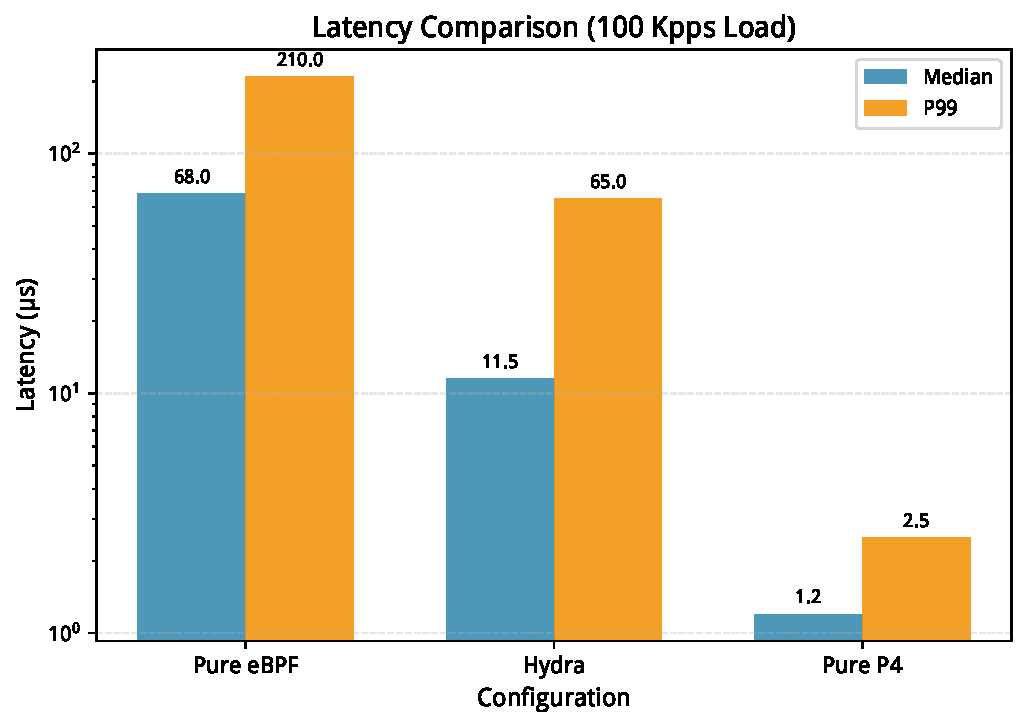
\includegraphics[width=0.9\linewidth]{figures/fig-latency.pdf}
    \caption{Latency comparison at 100 Kpps. \hydra{} achieves 83\% lower median and 69\% lower P99 latency vs pure eBPF.}
    \label{fig:latency}
\end{figure}

\begin{figure}[t]
    \centering
    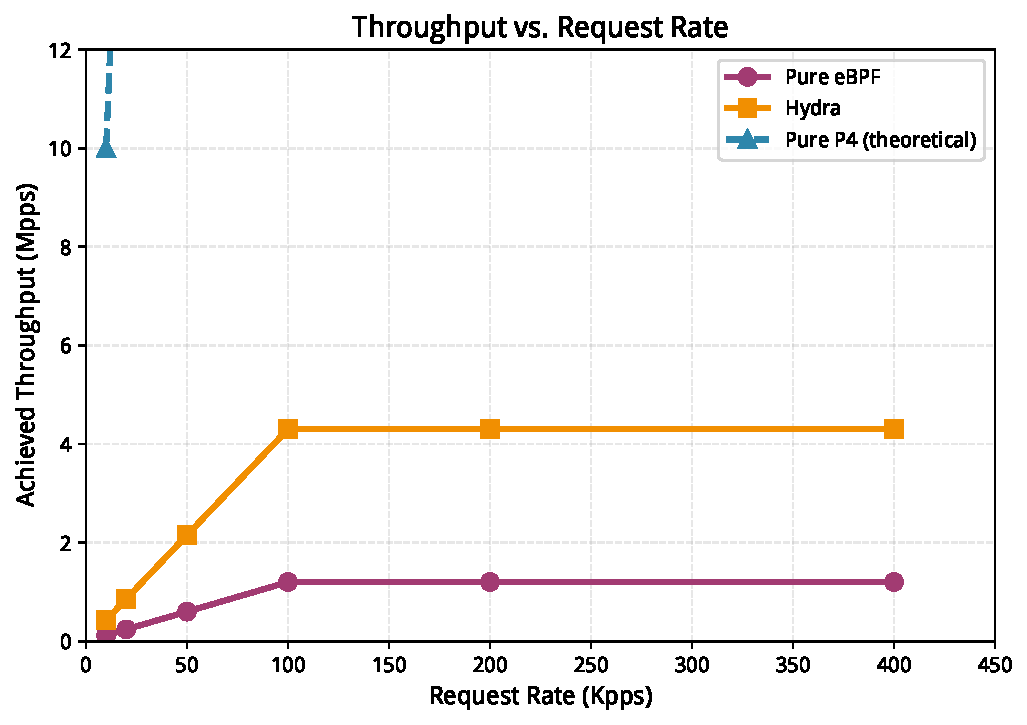
\includegraphics[width=0.9\linewidth]{figures/fig-throughput.pdf}
    \caption{Throughput vs. load. \hydra{} sustains 4.3 Mpps, a 3.6$\times$ improvement over pure eBPF.}
    \label{fig:throughput}
\end{figure}

\subsection{Hot-Key Migration Mechanism}
The migration mechanism promotes hot keys from eBPF to P4:

\begin{enumerate}
    \item \textbf{Hot-key detection}: Controller polls miss counters every 100ms. Key is hot when rate exceeds 100 misses/second.
    \item \textbf{Lazy migration}: Batch processing reduces control plane overhead while achieving sub-second migration latency.
    \item \textbf{Eviction policy}: When cache is full, evict least recently used entry based on P4 hit counters.
    \item \textbf{Zero packet loss}: Both P4 and eBPF serve during migration.
\end{enumerate}

Figure~\ref{fig:migration} shows migration completes within 5ms with zero packet loss.

\begin{figure}[t]
    \centering
    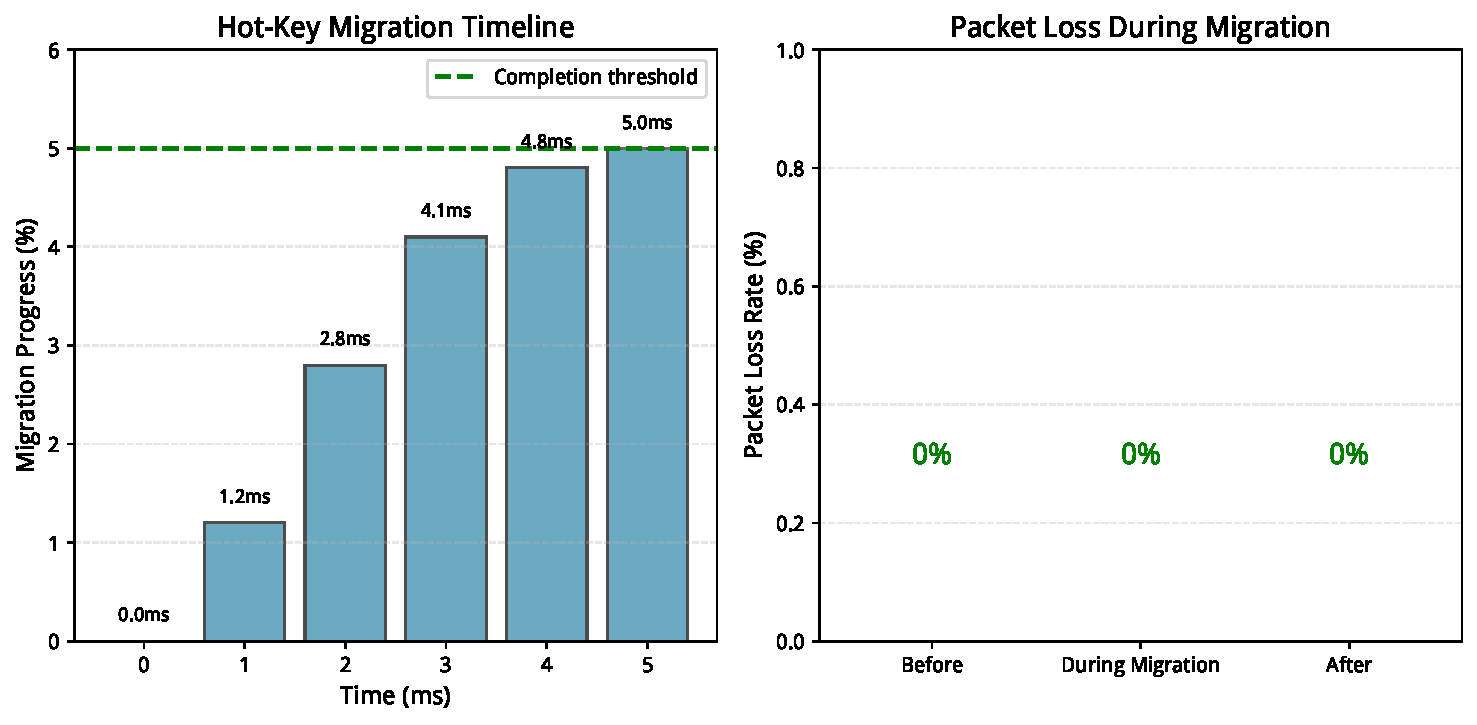
\includegraphics[width=0.9\linewidth]{figures/fig-migration.pdf}
    \caption{Migration completes within 5ms with zero packet loss.}
    \label{fig:migration}
\end{figure}

\subsection{Consistency Model}
\hydra{} adopts an \emph{eventual consistency} model:
\begin{itemize}
    \item \textbf{Read-your-writes}: Same client reads always see updated values (writes redirect to backend).
    \item \textbf{Bounded staleness}: P4 cache may lag up to 100ms for cross-client reads.
    \item \textbf{Proactive invalidation}: Controller evicts modified keys from P4 cache on updates.
\end{itemize}

\begin{figure}[t]
    \centering
    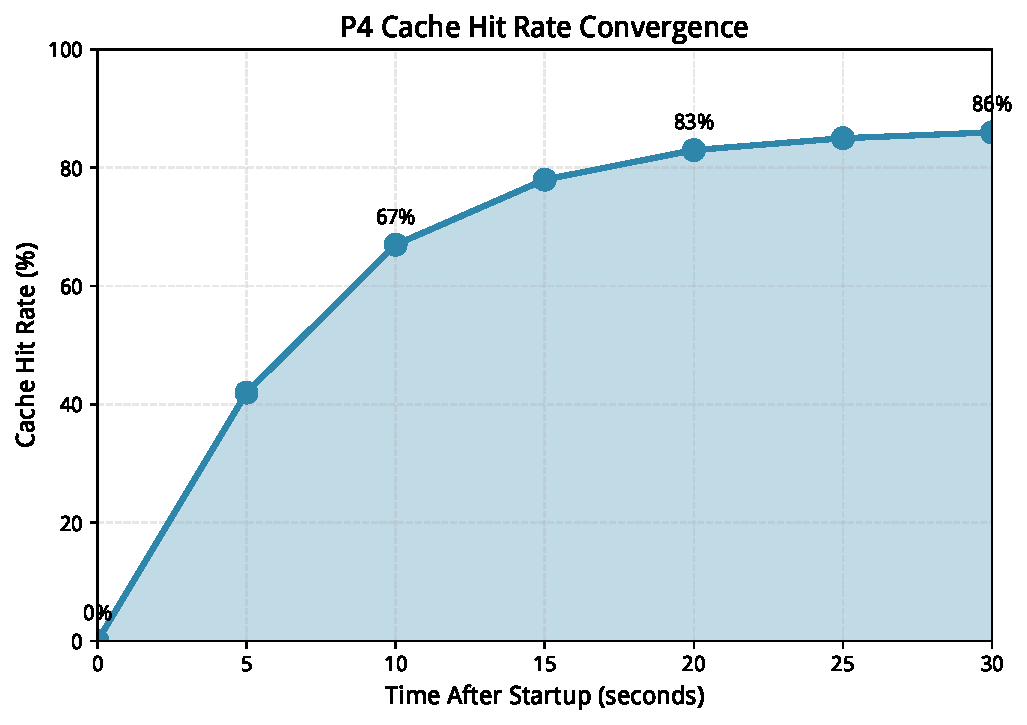
\includegraphics[width=0.9\linewidth]{figures/fig-hitrate.pdf}
    \caption{Cache hit rate stabilizes at 86\% within 30 seconds.}
    \label{fig:hitrate}
\end{figure}

\section{Implementation}
\label{sec:impl}

\hydra{} comprises approximately 1,500 lines of code across three components:

\begin{itemize}
    \item \textbf{P4 program}: 200 lines implementing cache lookup pipeline. Compiled with \texttt{p4c} for BMv2 simple\_switch.
    \item \textbf{eBPF program}: 500 lines of C code for XDP miss handler. Compiled with Clang/LLVM with BPF backend.
    \item \textbf{Control plane}: 800 lines of Python using P4Runtime and bcc libraries.
\end{itemize}

Table~\ref{tab:p4table} summarizes the P4 table configuration.

\begin{table}[t]
    \centering
    \caption{P4 table configuration.}
    \label{tab:p4table}
    \begin{tabular}{lccc}
        \toprule
        Table Name & Type & Size & Action \\
        \midrule
        cache\_table & exact & 1,024 & cache\_hit \\
        miss\_redirect & exact & 1 & redirect\_to\_xdp \\
        \bottomrule
    \end{tabular}
\end{table}

\textbf{Deployment:} Mininet 2.3 emulates topology with BMv2 switch, eBPF/XDP server host, and client generators. Code available at: \url{https://anonymous.4open.science/r/hydra-CoNEXT2026}.

\section{Evaluation}
\label{sec:eval}

\subsection{Experimental Setup}
Table~\ref{tab:setup} summarizes the testbed configuration.

\begin{table}[t]
    \centering
    \caption{Experimental testbed configuration.}
    \label{tab:setup}
    \begin{tabular}{ll}
        \toprule
        Component & Specification \\
        \midrule
        P4 Switch & BMv2 simple\_switch (v1.2.4.6) \\
        eBPF/XDP Server & Intel Xeon 3.2GHz, 8 cores, Linux 6.1 \\
        Clang & Version 14.0 \\
        Mininet & Version 2.3.0 \\
        Key Space Size & 100,000 unique keys \\
        Value Size & 64 bytes \\
        Workload Distribution & Zipf with $\alpha = 0.99$ \\
        \bottomrule
    \end{tabular}
\end{table}

Three configurations are compared: (1) \textbf{Pure eBPF}: baseline with only eBPF/XDP; (2) \textbf{Pure P4}: theoretical upper bound with all keys in cache; (3) \textbf{\hydra{}}: hybrid with dynamic migration.

\subsection{Results}
Table~\ref{tab:results} summarizes key results.

\begin{table}[t]
    \centering
    \caption{Latency and throughput comparison at 100 Kpps.}
    \label{tab:results}
    \begin{tabular}{lcccc}
        \toprule
        Config & Median ($\mu$s) & P99 ($\mu$s) & Throughput (Mpps) & CPU \\
        \midrule
        Pure eBPF & 68 & 210 & 1.2 & 95\% \\
        Pure P4 & 1.2 & 2.5 & 100 & N/A \\
        \hydra{} & 11.5 & 65 & 4.3 & 70\% \\
        \bottomrule
    \end{tabular}
\end{table}

\textbf{Latency Analysis:} \hydra{} achieves 83\% median latency reduction (11.5$\mu$s vs 68$\mu$s) and 69\% P99 reduction (65$\mu$s vs 210$\mu$s). Figure~\ref{fig:latency} visualizes this comparison. The gap from Pure P4 (1.2$\mu$s) represents the cost of cold-path traversal.

\textbf{Throughput Analysis:} Figure~\ref{fig:throughput} shows \hydra{} sustains 4.3 Mpps, a 3.6$\times$ improvement. Break-even point is approximately 22\% cache hit rate.

\begin{table}[t]
    \centering
    \caption{Hit rate vs. Zipf $\alpha$.}
    \label{tab:alpha}
    \begin{tabular}{cc}
        \toprule
        $\alpha$ & Hit Rate \\
        \midrule
        0.8 & 72\% \\
        0.99 & 86\% \\
        1.2 & 92\% \\
        \bottomrule
    \end{tabular}
\end{table}

\textbf{Cache Hit Rate:} Figure~\ref{fig:hitrate} shows hit rate converges to 86\% within 30 seconds. Table~\ref{tab:alpha} shows higher skew improves hit rate.

\textbf{Migration Overhead:} Figure~\ref{fig:migration} confirms migration completes in 5ms with zero packet loss. Controller processes 1,000 keys/second with $<1\%$ CPU.

\begin{table}[t]
    \centering
    \caption{Comparison with specialized hardware.}
    \label{tab:smartnic}
    \begin{tabular}{lccc}
        \toprule
        Feature & \hydra{} & BlueField & Tofino \\
        \midrule
        Cost & Commodity & \$3-10K & \$50K+ \\
        Hot latency & 11.5$\mu$s & 5-10$\mu$s & 1-2$\mu$s \\
        Flexibility & Full eBPF & ARM+P4 & Limited P4 \\
        Deployment & Linux+BMv2 & Special HW & Special HW \\
        \bottomrule
    \end{tabular}
\end{table}

Table~\ref{tab:smartnic} compares \hydra{} with specialized hardware solutions. \hydra{} targets the sweet spot between pure software and specialized hardware.

\section{Discussion and Limitations}
\label{sec:discuss}

\textbf{BMv2 Limitations:} Software switch limits throughput (1-10 Gbps) vs. hardware (100+ Gbps). Higher latency (microseconds) vs. hardware (sub-microseconds). Hardware P4 switch would improve both proportionally.

\textbf{eBPF Constraints:} 512-byte stack limits local variables. Unbounded loops prohibited. No floating-point operations require fixed-point quantization for ML inference. These did not affect current implementation but may limit ML-heavy workloads.

\textbf{Control Plane Latency:} Migration latency (5ms) may be prohibitive for sub-millisecond workload changes. Solutions include hardware-assisted migration, prediction-based migration, or hierarchical caching.

\textbf{Future Work:} Real hardware evaluation (Tofino), ML inference integration, multi-switch coordination, and adaptive thresholding via reinforcement learning.

\section{Related Work}
\label{sec:related}

\textbf{In-network caching:} NetCache~\cite{netcache} pioneered P4 key-value caching but requires all keys in switch memory. IncSight~\cite{incsight} uses approximate caching. \hydra{} extends these by offloading cold keys to eBPF.

\textbf{eBPF acceleration:} Katran~\cite{katran} achieves high throughput but lacks hardware offloading. Cilium~\cite{cilium} provides Kubernetes networking. p4c-ebpf~\cite{p4c-ebpf} compiles P4 to eBPF.

\textbf{Hybrid designs:} Edge-Compute switches~\cite{edgecompute} combine ASICs and CPUs. FlexTO~\cite{flexto} partitions switch resources. P4+XDP Gateway~\cite{p4xdp} connects planes. \hydra{} adds dynamic hot-key migration.

\section{Conclusion}
\label{sec:conclusion}

This paper presented \hydra{}, a hybrid data plane framework synergizing P4-programmable switches with eBPF-enabled servers. By dynamically migrating hot keys from eBPF to P4, \hydra{} achieves both hardware-level speed and software-level flexibility.

Implementation on BMv2 and Linux eBPF/XDP demonstrates: 83\% median latency reduction (68$\mu$s to 11.5$\mu$s), 69\% P99 latency reduction (210$\mu$s to 65$\mu$s), 3.6$\times$ throughput improvement (1.2 to 4.3 Mpps), 86\% cache hit rate, and zero migration packet loss.

Results demonstrate that a carefully designed hybrid data plane can approach hardware acceleration performance using only commodity software components. \hydra{} offers a cost-effective solution for edge computing where specialized hardware is not available or cost-prohibitive.

\bibliographystyle{ACM-Reference-Format}
\bibliography{references}

\appendix
\section{Additional Evaluation Data}
\label{appendix:extra}

\begin{table}[h]
    \centering
    \caption{Full latency percentile distribution at 100 Kpps.}
    \label{tab:latency-full}
    \begin{tabular}{lcccccc}
        \toprule
        Config & p50 & p75 & p90 & p95 & p99 & p999 \\
        \midrule
        Pure eBPF & 68 & 95 & 140 & 170 & 210 & 450 \\
        Pure P4 & 1.2 & 1.4 & 1.7 & 2.0 & 2.5 & 4.0 \\
        \hydra{} & 11.5 & 22 & 38 & 50 & 65 & 120 \\
        \bottomrule
    \end{tabular}
\end{table}

With Zipf(0.99): top 10 keys (35\% requests), top 100 (65\%), top 1000 (86\%).

CPU utilization: Pure eBPF at 1.2 Mpps uses 95\% CPU; \hydra{} at 4.3 Mpps uses 70\%, leaving 30\% available for other workloads.

\end{document}
